\providecommand{\main}{..}
\documentclass[main.tex]{subfiles}

\begin{document}
\chapter{Electronic Design}
\section{System Overview}

The electronic hardware of the system was designed according to the following principles, decided upon early in the project:
\begin{enumerate}
    \item The design shall be modular and will allow for adjustments in any stage of the design with minimal impact on the board as a whole.
    \item The design shall incorporate a general purpose, WiFi enabled companion computer.
    \item End-user input shall be limited to basic functionality, with no access to circuitry required for normal operation.
    \item The design shall incorporate verified circuitry where possible through the use of open-hardware COTS designs and application specific design tools.
\end{enumerate}
As a result of these, the final (1st generation) system took the form seen in \textit{Figure \ref{fig:electronics-system}}, featuring a Raspberry Pi Zero Wireless companion computer, a stereo audio DAC, a Class-D stereo amplifier, and several DC/DC power regulators. The required external connections were limited to a wall-mount 12V DC power supply, with several buttons for user input and a toggle switch for on/off control.

\begin{figure}[H]
    \centering
    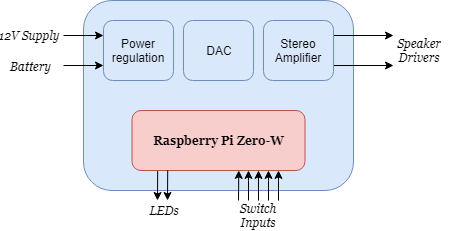
\includegraphics[scale=0.75]{./figs/electronics-system.png}        
    \caption{Electronics hardware overview}
    \label{fig:electronics-system}
\end{figure}

\section{Audio Stage}

Further requirements and desired features in the audio design were set early in the project, namely:
\begin{itemize}
    \item The system shall utilise a Class-D audio amplifier (a remnant of the original project brief to design/build/test a 100W Class-D amplifier).
    \item The system shall be a bi-amp design, removing the requirement for hardware crossover filtering which shall instead be achieved through software. 
    \item The audio stage shall accept an $I^{2}S$ digital audio input from the companion computer and $I^{2}C$ communication for hardware control.
    \item Each driver shall have an amplification stage on the order of $\approx20W RMS$.
\end{itemize}

The resultant configurations from these requirements were then reduced to two choices: to have separated Digital-to-Analog conversion and Amplification stages, or to utilise a combined digital input amplifier, each presenting advantages and drawbacks.
\par
A fully integrated system presents decreased BOM count and design effort - and greater immunity to noise - at the expense of setup requirements. Modern single-stage ICs offer far greater on-chip signal processing abilities but require a far more sophisticated control scheme because of it, and often rely on evaluation modules to ease their development. 
\par
A dual stage system is fundamentally worse in matters of signal integrity, and offers few advantages in this regard. In contrast to single stage systems however they provide far more choice in control complexity between each stage, and allow for the selection of ICs already in use within cheap COTS expansion modules. The advantage presented by this is the use of these COTS modules for software and audio development in parallel with electronic design, with the completed electronic system then seamlessly replacing the development setup upon completion.
\par
As both of these approaches offered interesting areas of investigation they were decided to both be pursued. The initial system would utilise the advantages of the verified dual stage system and provide a guaranteed performance of the final system. The single stage system would then be developed afterwards with a lower priority, and would present room for comparison between the classical and modern design methodologies. To reduce complexity in the overall design and bring-up components were selected such that each of the systems would have identical power stages and overall board design.

\subsection{1st Generation Dual-Stage Board}

The initial system designed can be seen in \textit{Figure \ref{fig:audio-system}}, with components selection governed by the availability of compatible COTS modules. 

\begin{figure}[H]
    \centering
    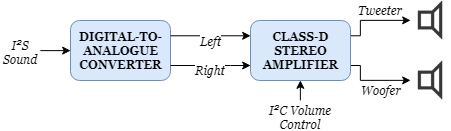
\includegraphics[scale=0.75]{./figs/audio-system.png}
    \caption{Dual stage audio system}
    \label{fig:audio-system}
\end{figure}

\subsubsection{DAC}
The initial module selected for development of the streaming software was the Pimoroni pHAT DAC, based on the Texas Instruments PCM5102A audio stereo DAC. This board not only met the hardware requirements, but as a dedicated expansion board for the Pi Zero W provided device tree setup and software libraries which expedited testing. The board layout and component choice both conformed to the recommended application information provided within the component datasheet, and thus could be reliably replicated, as seen in \textit{Figure \ref{fig:dac-circuit}}.

\begin{figure}[H]
    \centering
    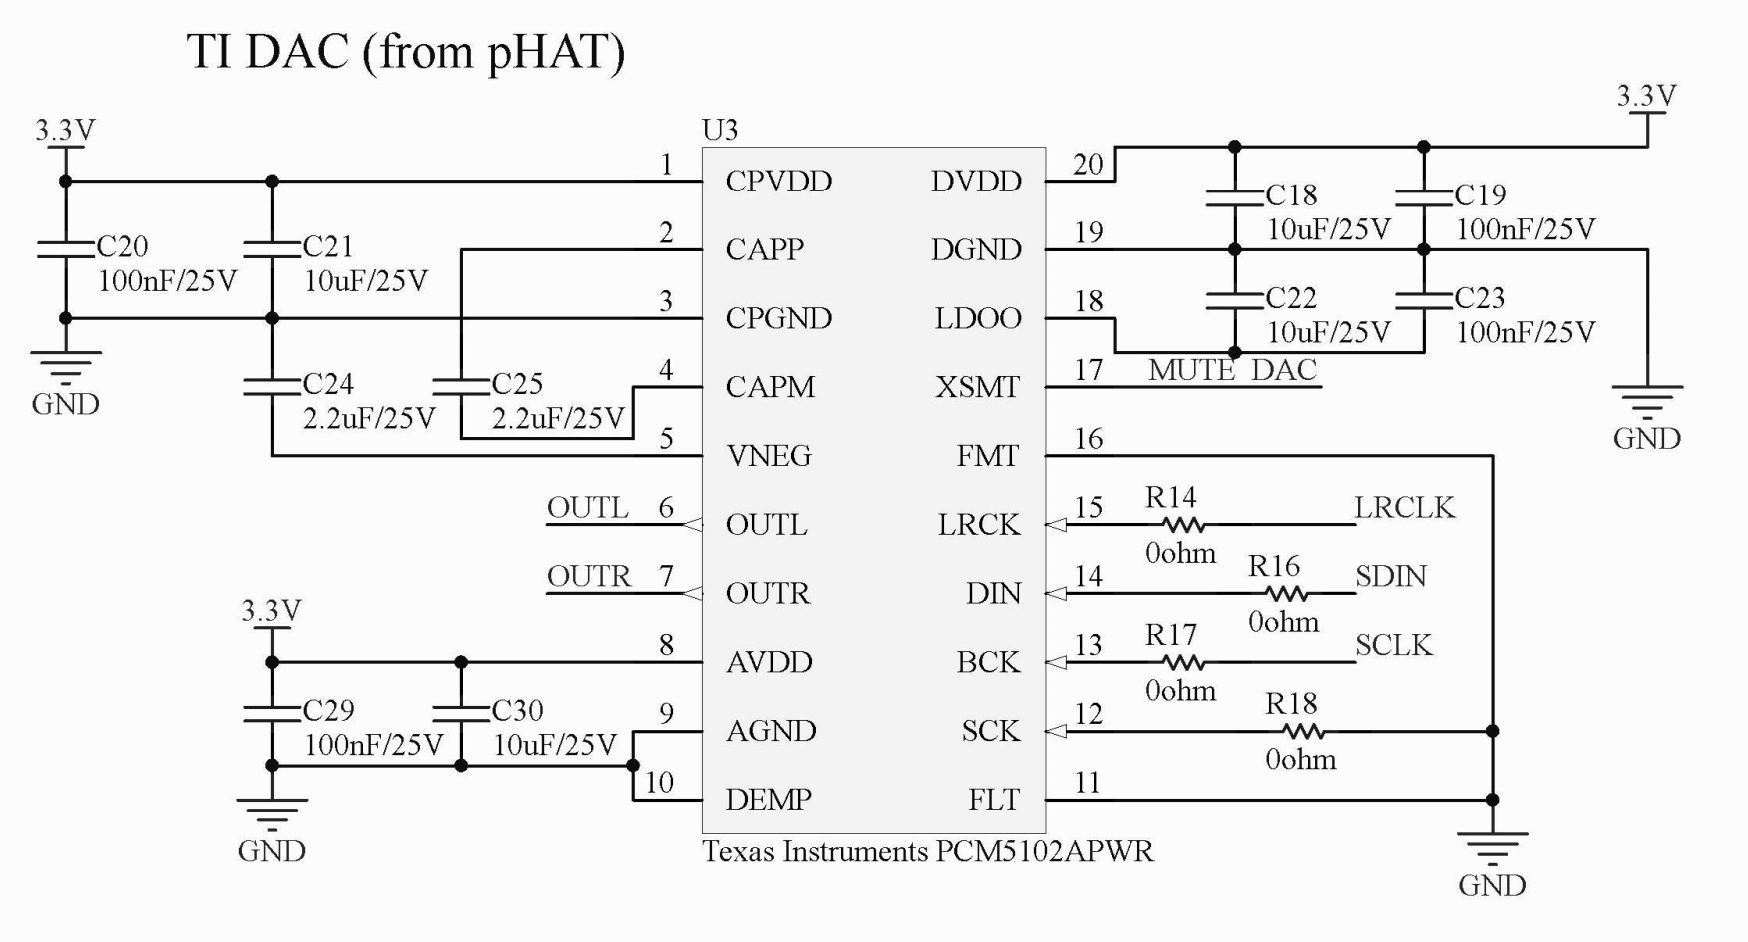
\includegraphics[scale=0.6]{./figs/DAC-circuit.PNG}
    \caption{DAC schematic}
    \label{fig:dac-circuit}
\end{figure}

\subsubsection{Amplifier}
The amplifier stage selection was governed by the desire for low control complexity and low BOM cost while maintaining the aforementioned requirements. The Maxim Integrated MAX9744 fit these criteria with the advantage of its use in a range of commercial designs. The required control is limited to the volume selection by setting a single register value, and its capability to use ferrite beads on its outputs at the operating condition desired removed the significant cost power inductors present. As shown in \textit{Figure \ref{fig:maxim-circuit}}, the recommended schematics and layouts provided in the device datasheet were again used. Hardware analog control was disabled and 100nF decoupling capacitors added alongside the bulk capacitance on the power supply pins.

\begin{figure}[H]
    \centering
    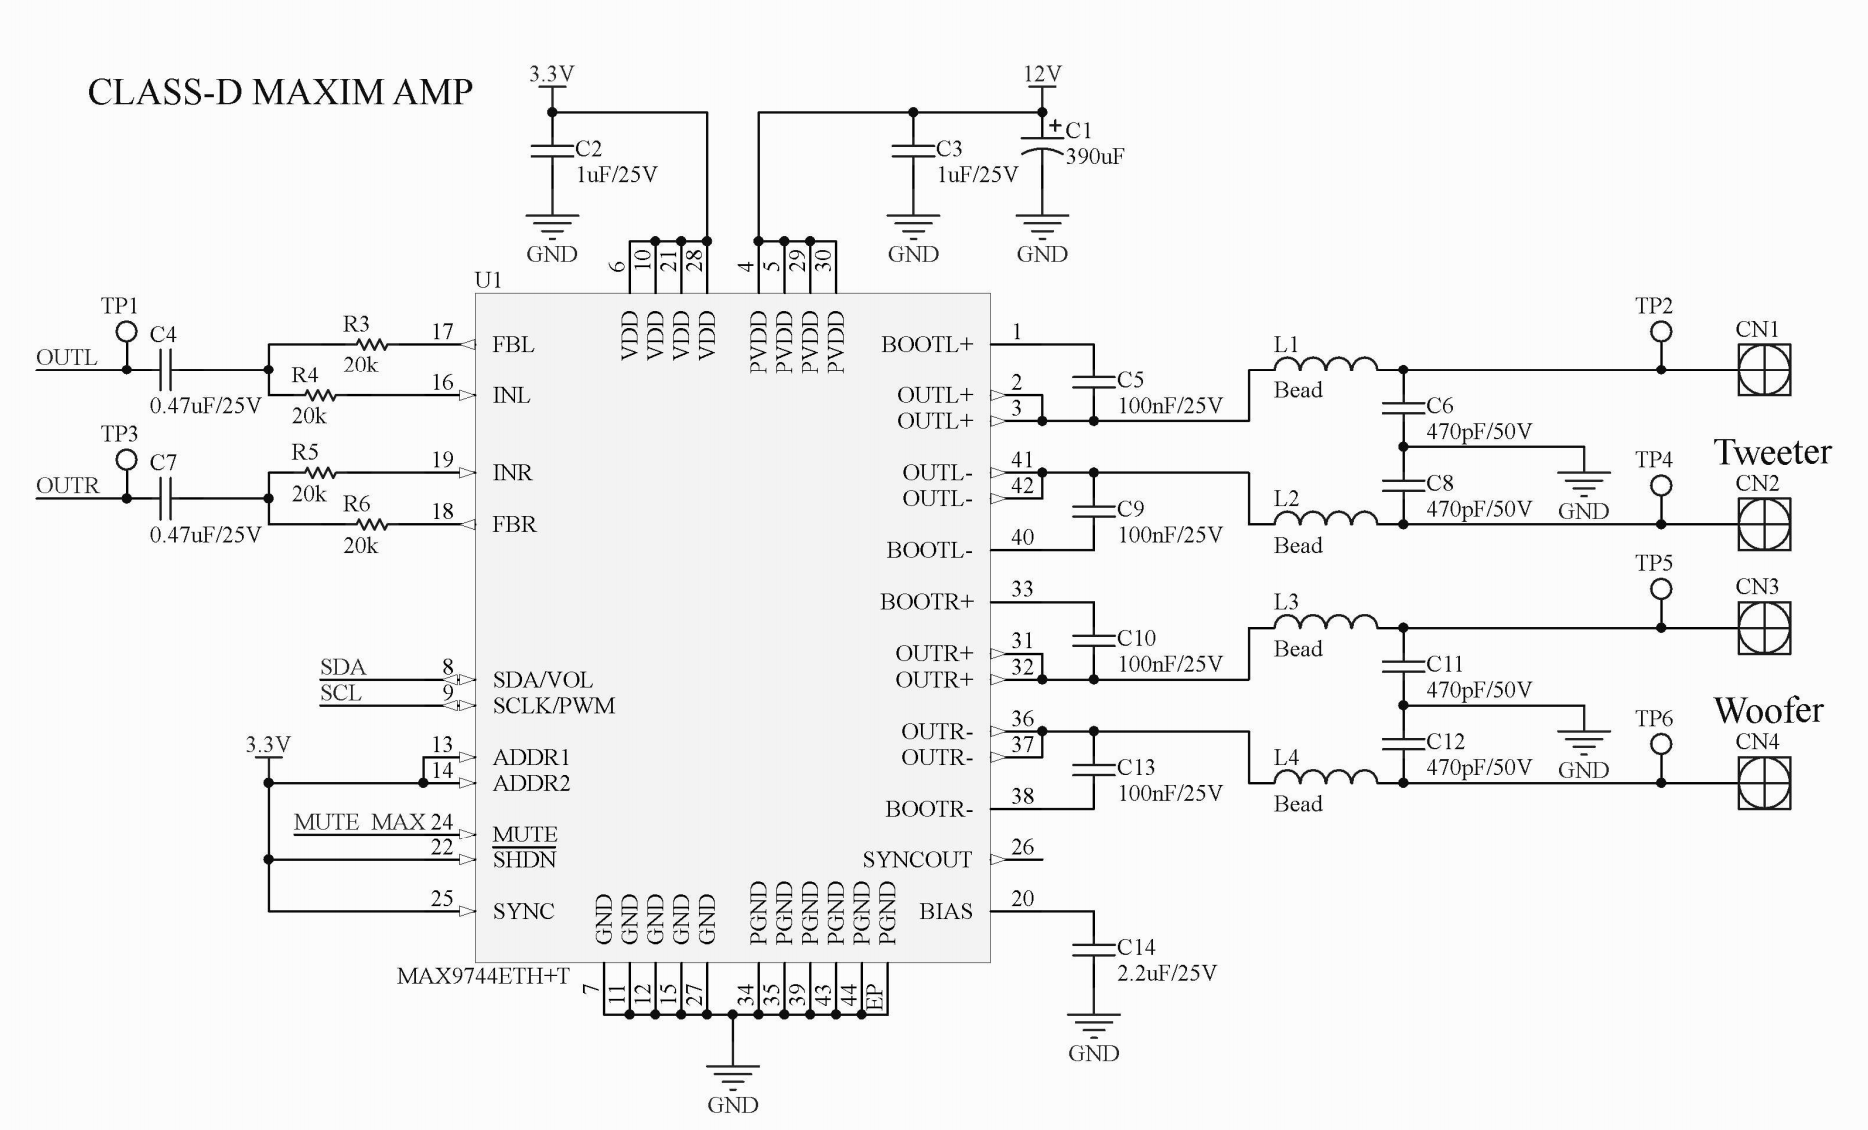
\includegraphics[scale=0.6]{./figs/MAXIM-circuit.PNG}
    \caption{Amplifier schematic}
    \label{fig:maxim-circuit}
\end{figure}

\subsection{2nd Generation Single-Stage Board}

\begin{figure}[H]
    \centering
    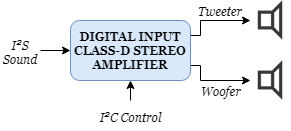
\includegraphics[scale=0.75]{./figs/TAS-system.png}
    \caption{Single stage audio system}
    \label{fig:tas-system}
\end{figure}

For subsequent development of the fully integrated system a digital input amplifier was selected based on its conformance to the project requirements as well as the previously generated power supply. The result of this was the Texas Instruments TAS5805M, a far more modernised IC than those in the dual system, capable of accepting the same $I^S$ signal and $I^2C$ control signal while incorporating a number of DSP capabilities. The produced schematic can be seen in \textit{Figure \ref{fig:tas-circuit}} and worked as desired barring the lack of address-setting resistor due to an error in design.

\begin{figure}[H]
    \centering
    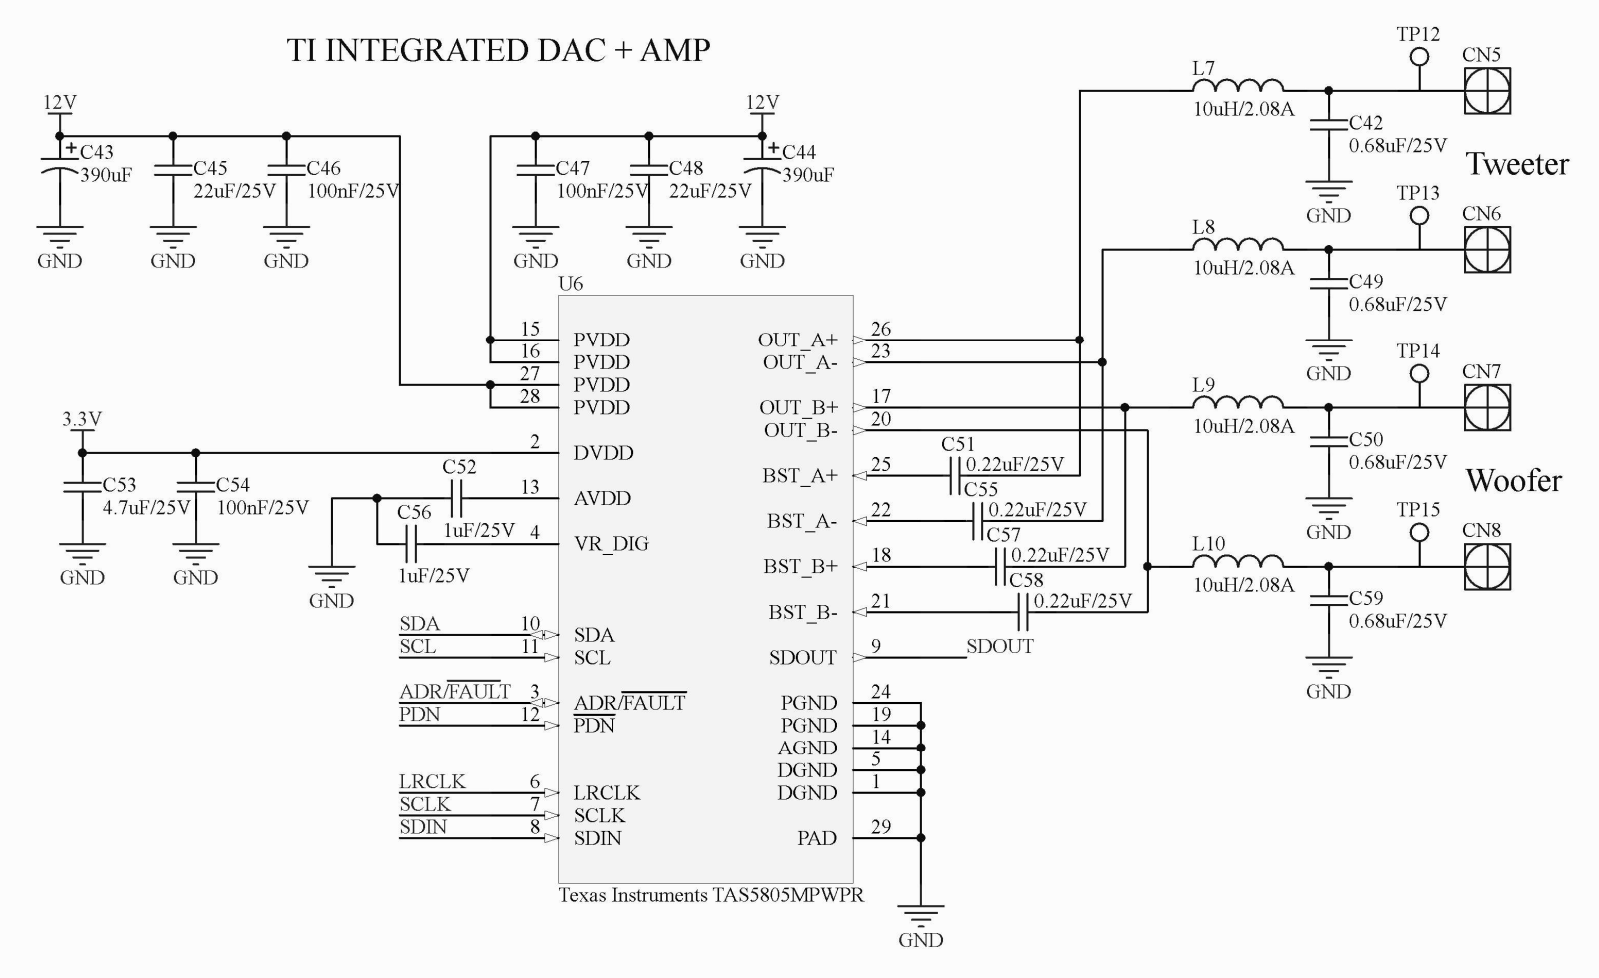
\includegraphics[scale=0.75]{./figs/TAS-circuit.PNG}
    \caption{Digital input amplifier schematic}
    \label{fig:tas-circuit}
\end{figure}

Initial configuration of the device was achieved by using the Texas Instruments PurePath Configurator 3 software to generate configuration header files. An array of $I^2C$ addresses and commands was produced providing the required register values and page navigation of the device, .

\section{Power Stage}

To power the system three regulated outputs were required. The amplifier power inputs were supplied by a 12V rail, a 5V rail powered the companion computer, and a final 3.3V supply provided the logic level power for the board ICs. The system was then selected utilising the Texas Instrument Webench power designer prioritising for BOM cost and footprint area. Two TI TPS62135 buck regulating DC/DC converters were chosen to generate the 12V (from unregulated battery power) and 5V high power rails, with a TI TLV70033 LDO regulator provided the low current requirement logic level supply. 

\begin{figure}[H]
    \centering
    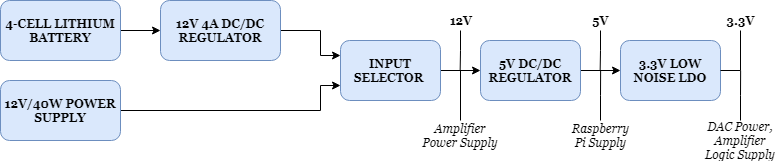
\includegraphics[scale=0.6]{./figs/power-system.png}
    \caption{Power regulation electronics}
    \label{fig:power-system}
\end{figure}

To avoid the risk presented by mains power regulation the speakers were designed such that the user faced only a 12V $\approx$ 40W power supply sourced from a validated supplier. This was chosen as the XP Power VEL36US120-UK-JA, a generic COTS supply fit for the purpose which, while being rated only for 36W, fit the desired form factor and cost required to be seen as an acceptable risk.

\begin{figure}[H]
    \centering
    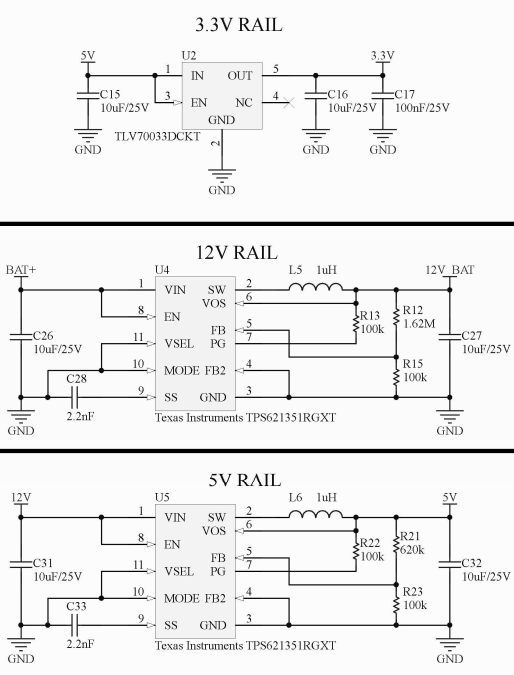
\includegraphics[scale=1.2]{./figs/power-circuit.PNG}
    \caption{Power regulation schematic}
    \label{fig:power-circuit}
\end{figure}

\subsubsection{Design Considerations}

Although the system design was largely governed by the Webench designer and datasheet applications small changes were made to the system to incorporate good-practice procedures. Power inputs and outputs on each subsystem were decoupled with 100nF transient suppressing capacitors as well as a local bulk capacitance. Any MLCCs (multi-layer ceramic capacitors) used were rated for 25V to reduce their large derating seen around the rated voltage, and extra footprints for bulk capacitance placed around the board. 

\subsection{Battery Power}

To incorporate the desire for the system to operate in a truly wireless sense circuitry was added to provide for the regulation and selection of a 4-cell lithium battery power supply. A P-type FET placed in series with the regulated battery output switched the supply off based on the insertion of the DC barrel jack providing wall-power, and vice-versa. As the system was only for test and not a requirement of the device protection and charging circuitry was not provided. 

\section{PCB Design}

Schematic capture and PCB design were both produced in Altium's community oriented Circuitmaker software. Components were selected based on their availability at preferred suppliers - namely Onecall - and selected in the design using the platforms OCtopart component database integration. This method allowed for both the use of community generated footprints as well as the generation of supplier specific BOMs for purchasing. 

\subsection{Test Boards}
To allow for design verification and early testing PCBs were fabricated containing each of the audio stages. These boards were build to 
%%%INITITAL TEST PCBS

\subsubsection{Layout}

Placement of components and passives closely followed the recomment layous given in their respective datasheet, with each block placed into its respective audio, power, or debug board regions. 

\begin{figure}[H]
    \centering
    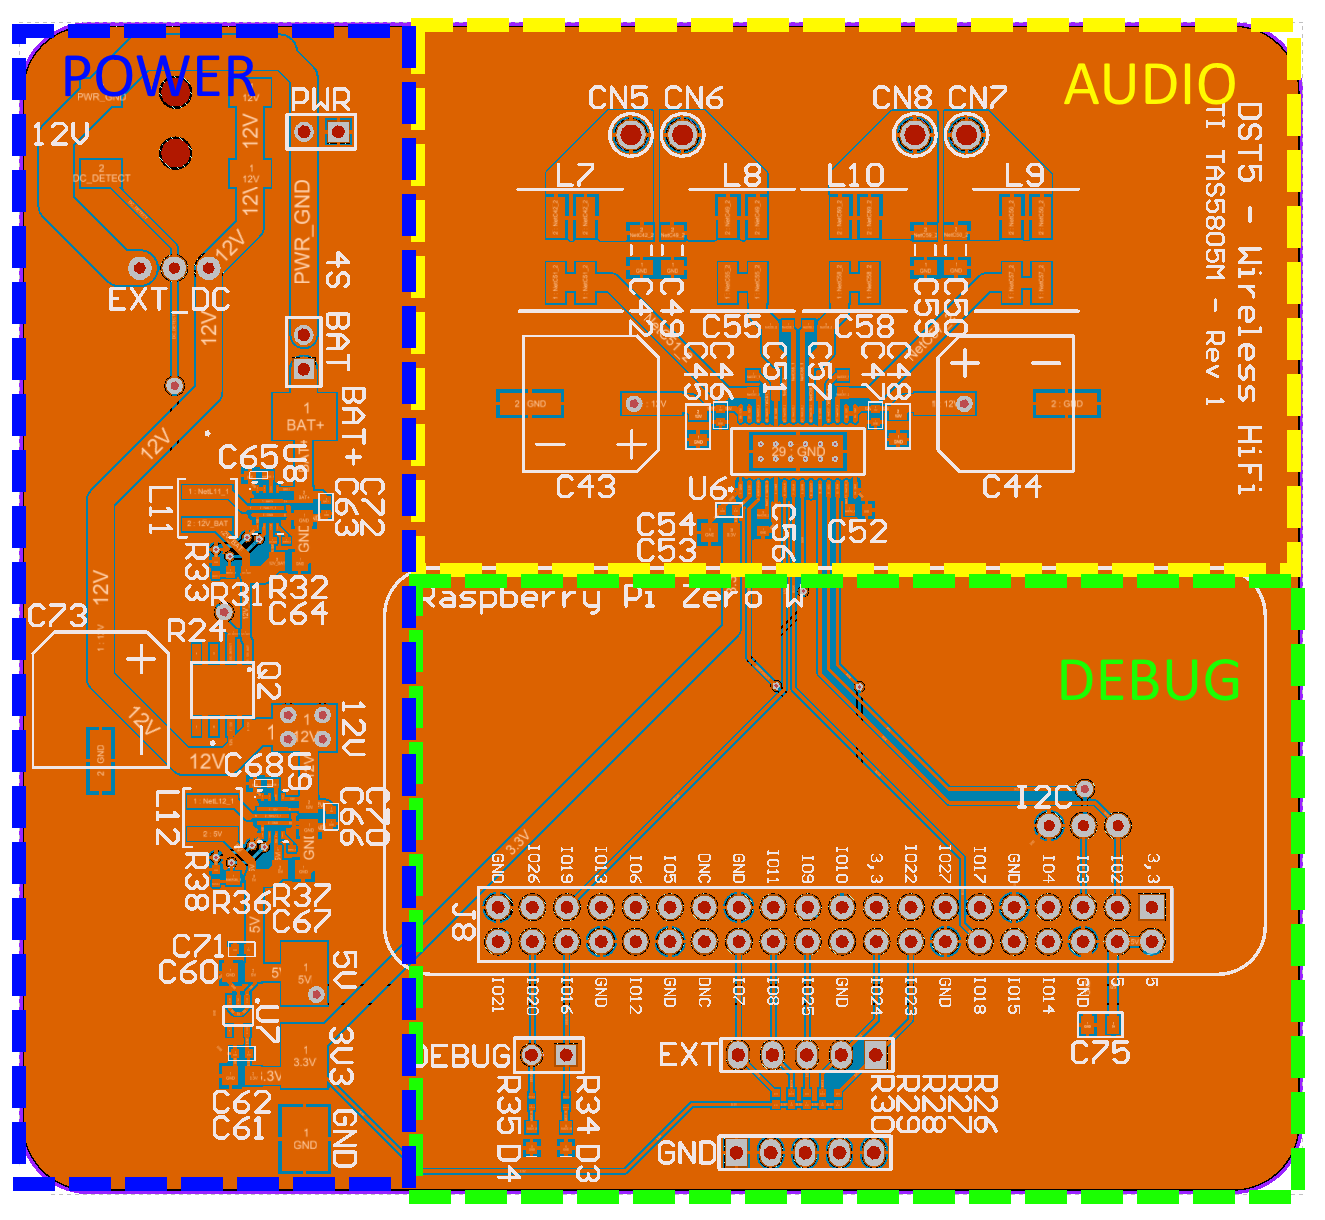
\includegraphics[scale=0.4]{./figs/ti-pcb.png}
    \caption{Single stage board layout}
    \label{fig:ti-pcb}
\end{figure}

\subsubsection{Fabrication}



\section{User I/O}
\section{Testing}
\subsection{Overview}
\subsection{Results}
\end{document}